% tbp-double on Cu(111)
When depositing trans-TBP on Cu(111) at room temperature no strict ordering can be achieved. The molecules arrange rather arbitrarily as can be seen in figure \ref{fig:two-leg-trans-cu111}.

\begin{figure}[h]
 \centering
 \subfigure[]{
 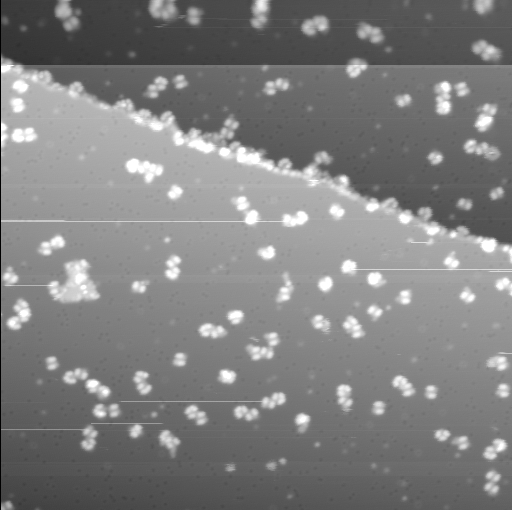
\includegraphics[width=0.3\textwidth]{./images/F160425-172349.png}
 }
 \subfigure[New preparation adsorbed at \SI{70}{\celsius}]{
 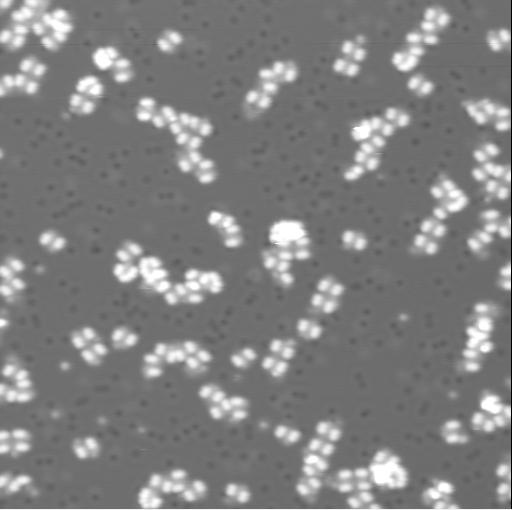
\includegraphics[width=0.3\textwidth]{./images/F160427-121720.png}
 }
 \subfigure[... and heated for \SI{10}{\minute} to \SI{170}{\celsius}]{
 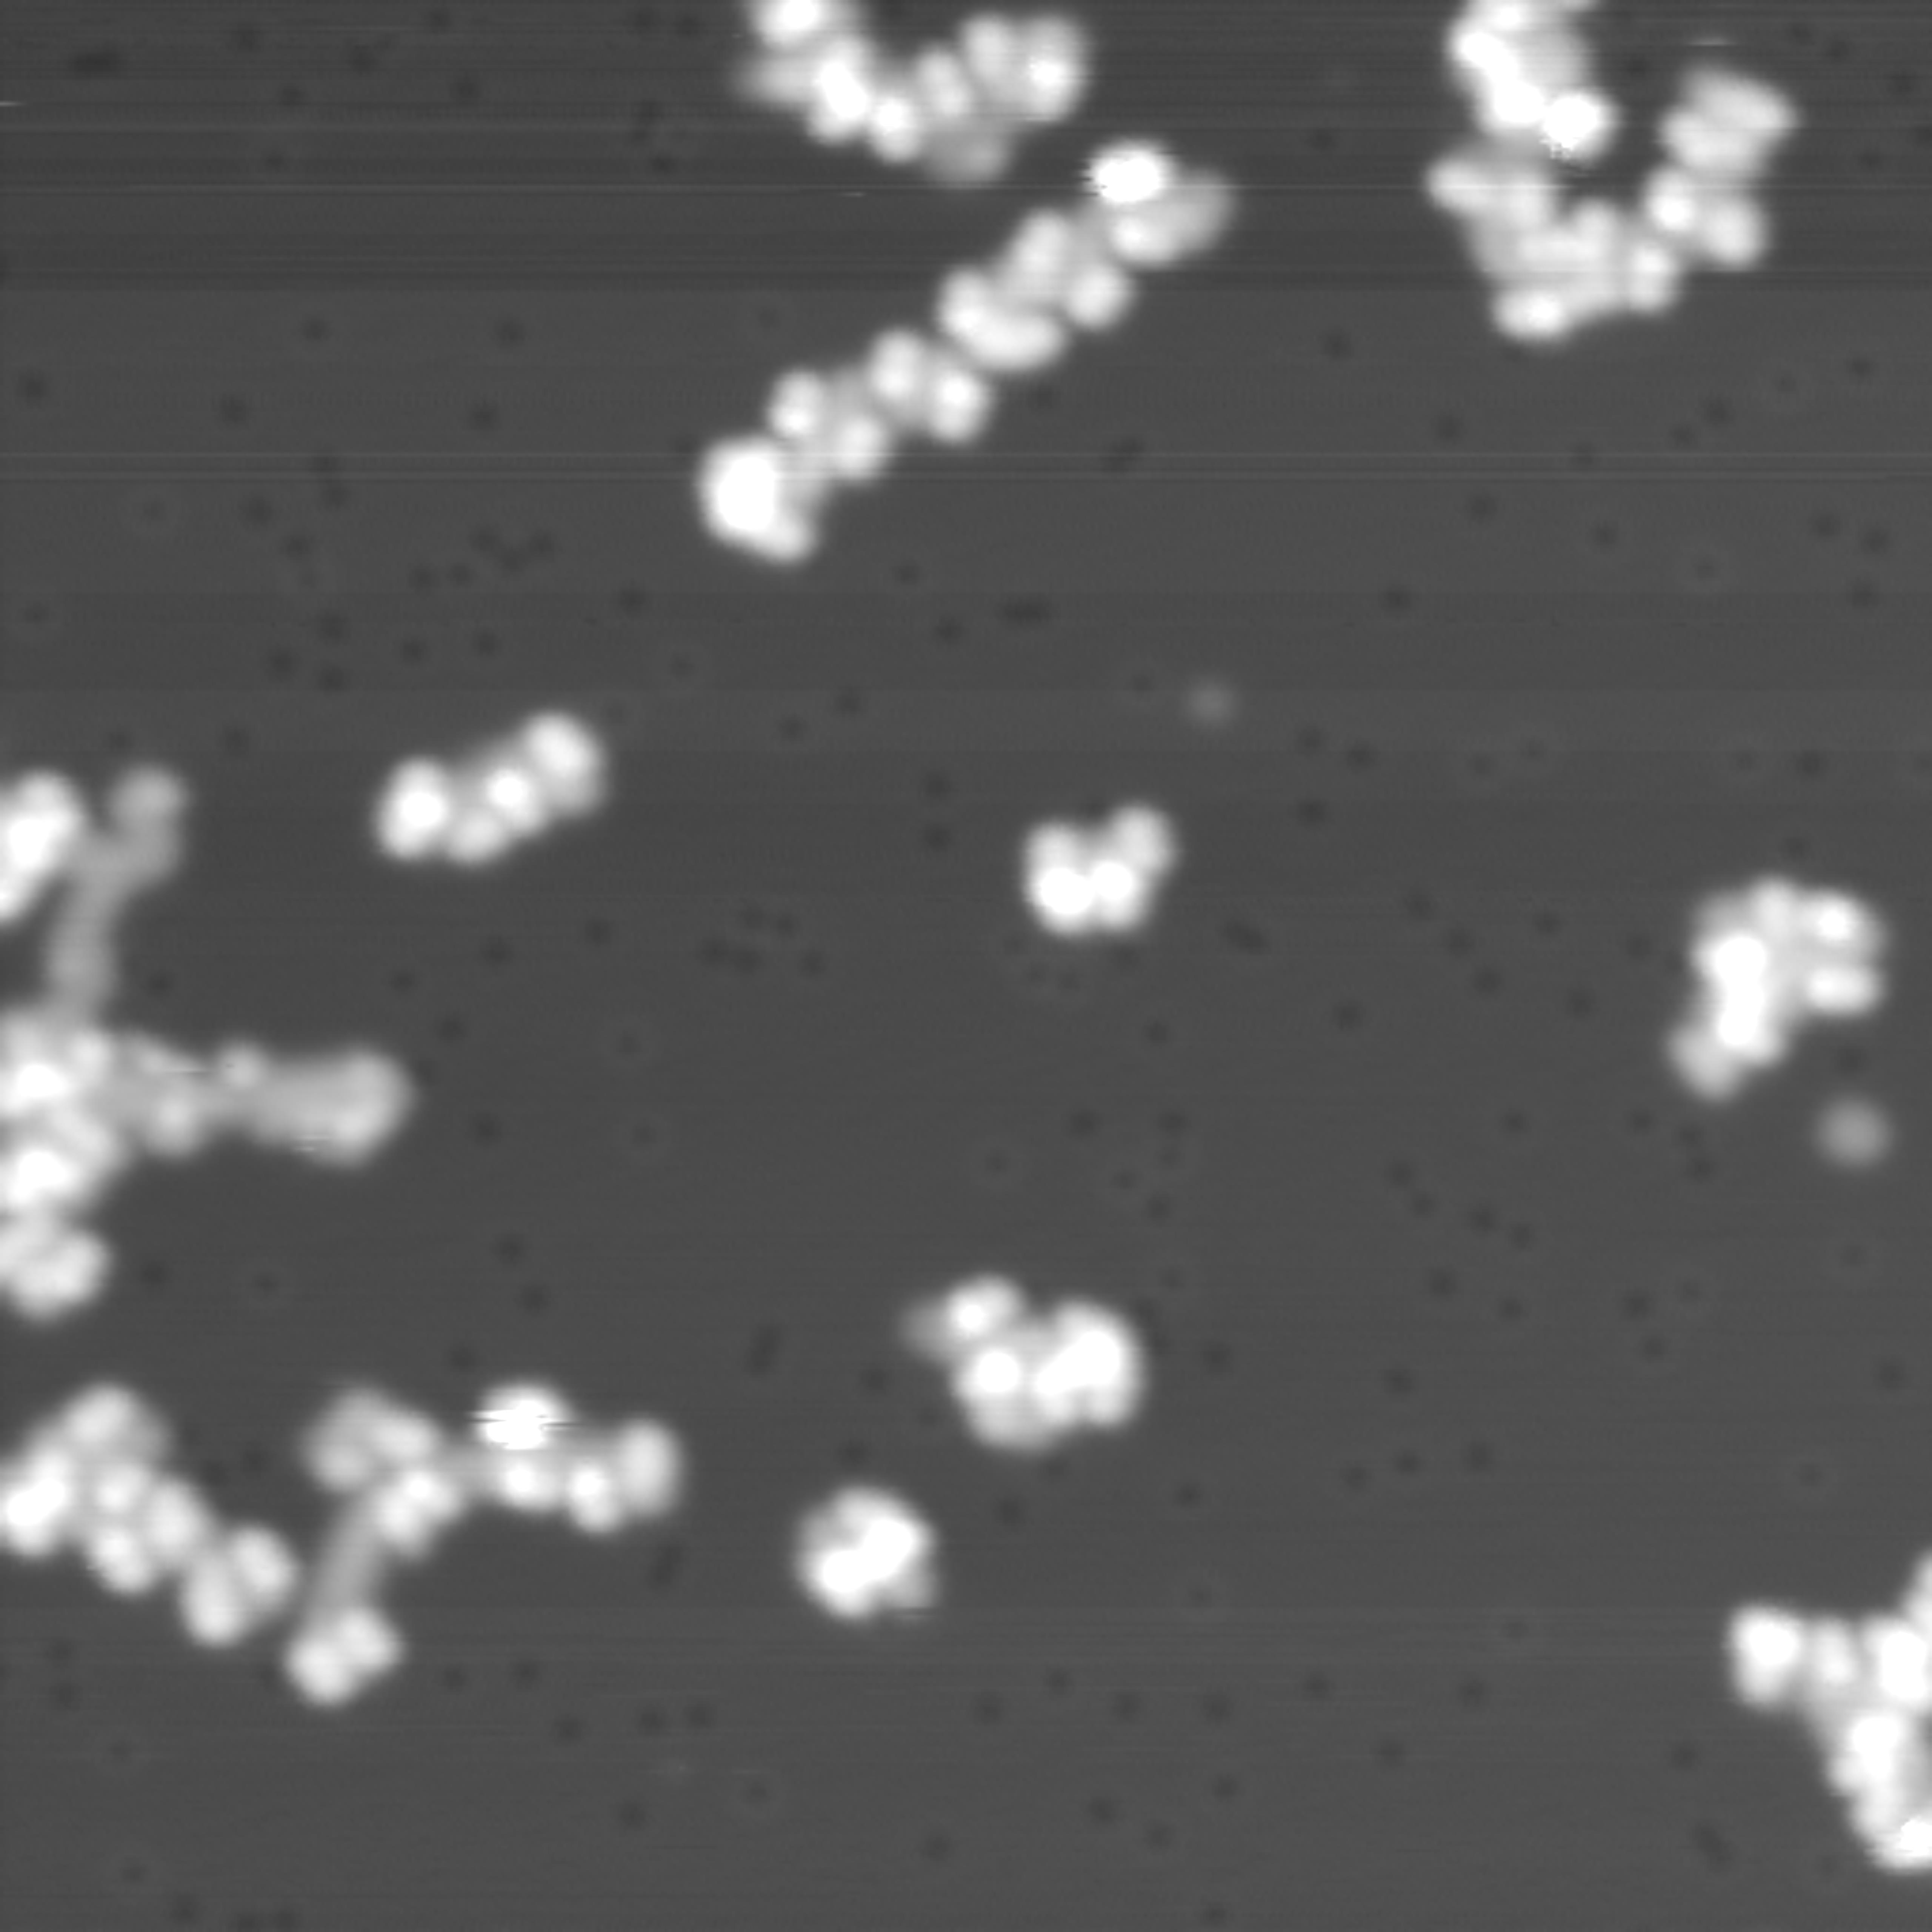
\includegraphics[width=0.3\textwidth]{./images/F160428-162039.png}
 }
\caption{Molecules adsorbed on Cu(111) at different temperatures. Adsorption at room temperature (a) did not show extended long range order. Adsorption at \SI{70}{\celsius} (b) and heating to \SI{170}{\celsius} for \SI{10}{\minute} (c) improves the chain lenght sligthly.}
\label{fig:two-leg-trans-cu111}
\end{figure}

The molecules tend to connect in a difined angle to its next neighbour, forming different binding motivs. These are predominantly different kind of chain formation (see figure \ref{fig:two-leg-trans-cu111-motivs}).
\begin{itemize}
 \item The molecules are ordered such that they form a straight chain (trans-nitro-on-cu111-70).
 \item The molecules arrange in chains, but each molecule has an offset of about a half of its width to the next neighbour or the molecules attach in chains, but show a kink.
\end{itemize}

\begin{figure}[h]
 \centering
 \subfigure[Straight chain, Image width 15\,nm, every second molecule is rotated by 180\,degree around the x-axis (in plane with the image - create chiral molecule adsoprtion) to match the image best.]{
 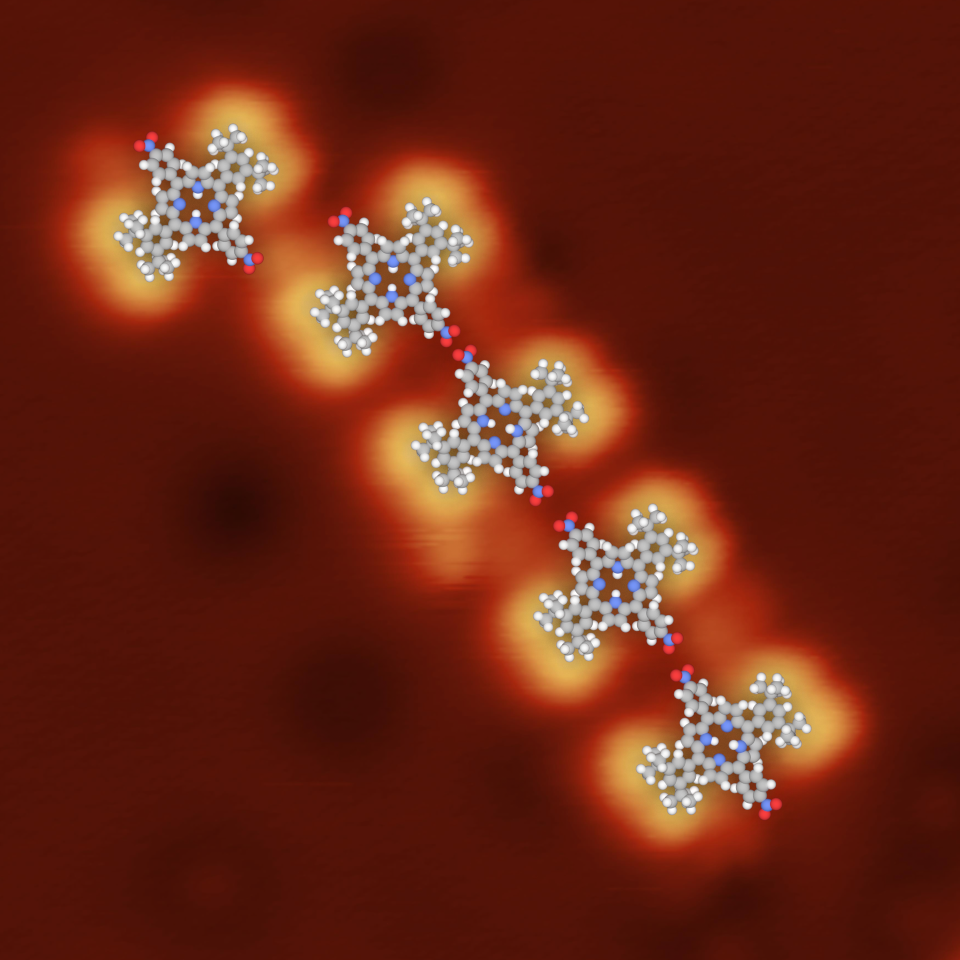
\includegraphics[width=0.45\textwidth]{./images/trans-nitro-on-cu111-70.png}}
 \subfigure[offset-chain interrupted by a kinked edge, image width again 15\,nm]{
 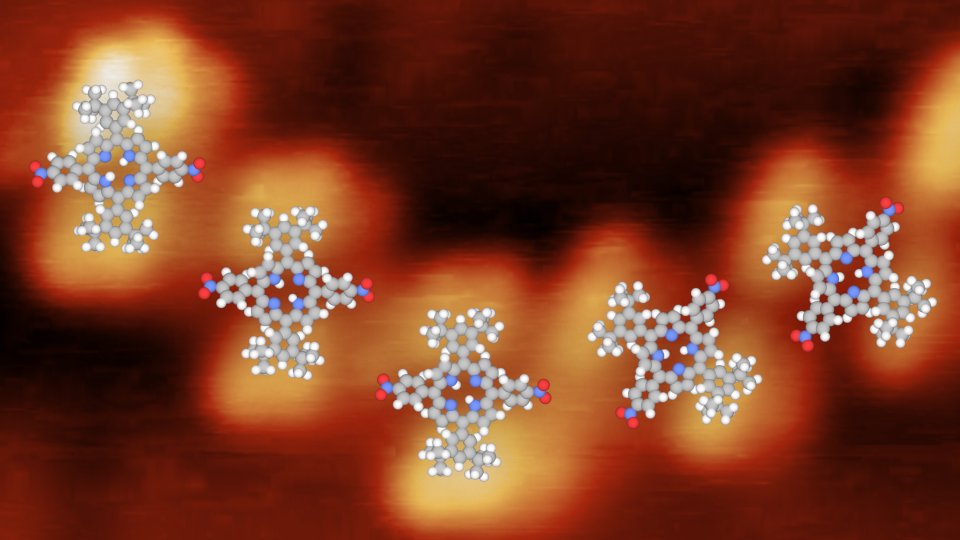
\includegraphics[width=0.45\textwidth]{./images/trans-nitro-on-cu111-120.png}}
\caption{All motives exist at every temperature, although the chain lenght increases with temperature. It also looks like the chains are getting more offset- and kinked-like chains than at lower temperatures.}
\label{fig:two-leg-trans-cu111-motivs}
\end{figure}

During modelling figure \ref{fig:two-leg-trans-cu111-motivs} the molecules are shown in their non interacting geometry. Note that every second molecule (in the model) is rotated by \SI{180}{\degree} to match the image best (one can see an repeating pattern where two adjacent molecules' butyl groups are alternating between two distances - either further away on one side and closer on the other side of the chain or vice versa). One can see, that their butyl-group nicely match the image in size and position when rotated. 

Having a closer look to the nitro groups, one recognizes a close proximity of these to each other. Also note the light protrusions in between two adjacent molecules' butyl groups. If the legs are rotaded by just \SI{15}{\degree}, the nitro groups would point to these protrusions. This rotation costs not much energy and is about \SI{25}{\kilo\J/per\mol} (( please cite something, value is for rotated phenyl ring at a porphine core I guess )). Considering these protrusions as Cu-adatoms (already occured in chapter \ref{chapter:TPCN-adatoms} as protrusions in between TPCN chains which may change their position in discrete position in the molecule.) This Cu-adtom may direct the binding of the nitro groups towards it, making them bend outwards. The position of the cooper atom itself may rely on its registry to the substrate - preferring a threefold coordination site as known for copper (( citation )).

